\documentclass[letter paper, title page]{article}
\usepackage{graphicx} % Required for inserting images
\usepackage[capposition=top]{floatrow}
\usepackage[margin=1in]{geometry}
\usepackage[export]{adjustbox}
\usepackage{tabularx}
\usepackage{multirow}
\usepackage{amssymb}

\title{\huge Physics 55 - Lab 4: Projectile Motion}
\author{Andrew Card, Preston Kearnan, Roan Morgan, Michael Roberts}
\date{February, 9 2023}

%the ball leaves the device at like 100 - (80.5cm) [19.5 = initial height]


\begin{document}
\maketitle

\section*{Muzzle Speed} %NEED QUESTIONS ANSWERED AND A TABLE OF VALUES & MEASUREMENTS
\title{Objective} 
\begin{list}
    \\ \item - We will learn how to apply projectile motion equations measuring the velocity of a metal ball shot out of a launcher. We will then record and plug this info into a tracker app in order to find our exact initial velocity. Later this will be used to accurately shoot a ball into a soup can first try.
\end{list}

\subsection*{Vertical Launch}

\noindent
\title{Synopsis}

\begin{list}
     \\ \item - We will first arrange the projectile launcher in a position that shoots the ball upwards. 
      \item - We will record ourselves shooting the ball upwards with a meter stick in order to measure the height the ball is launched.
    
      \item- We will then make a calculation to find the initial velocity of the ball. 
\end{list}

\begin{figure}[H]
    \centering
    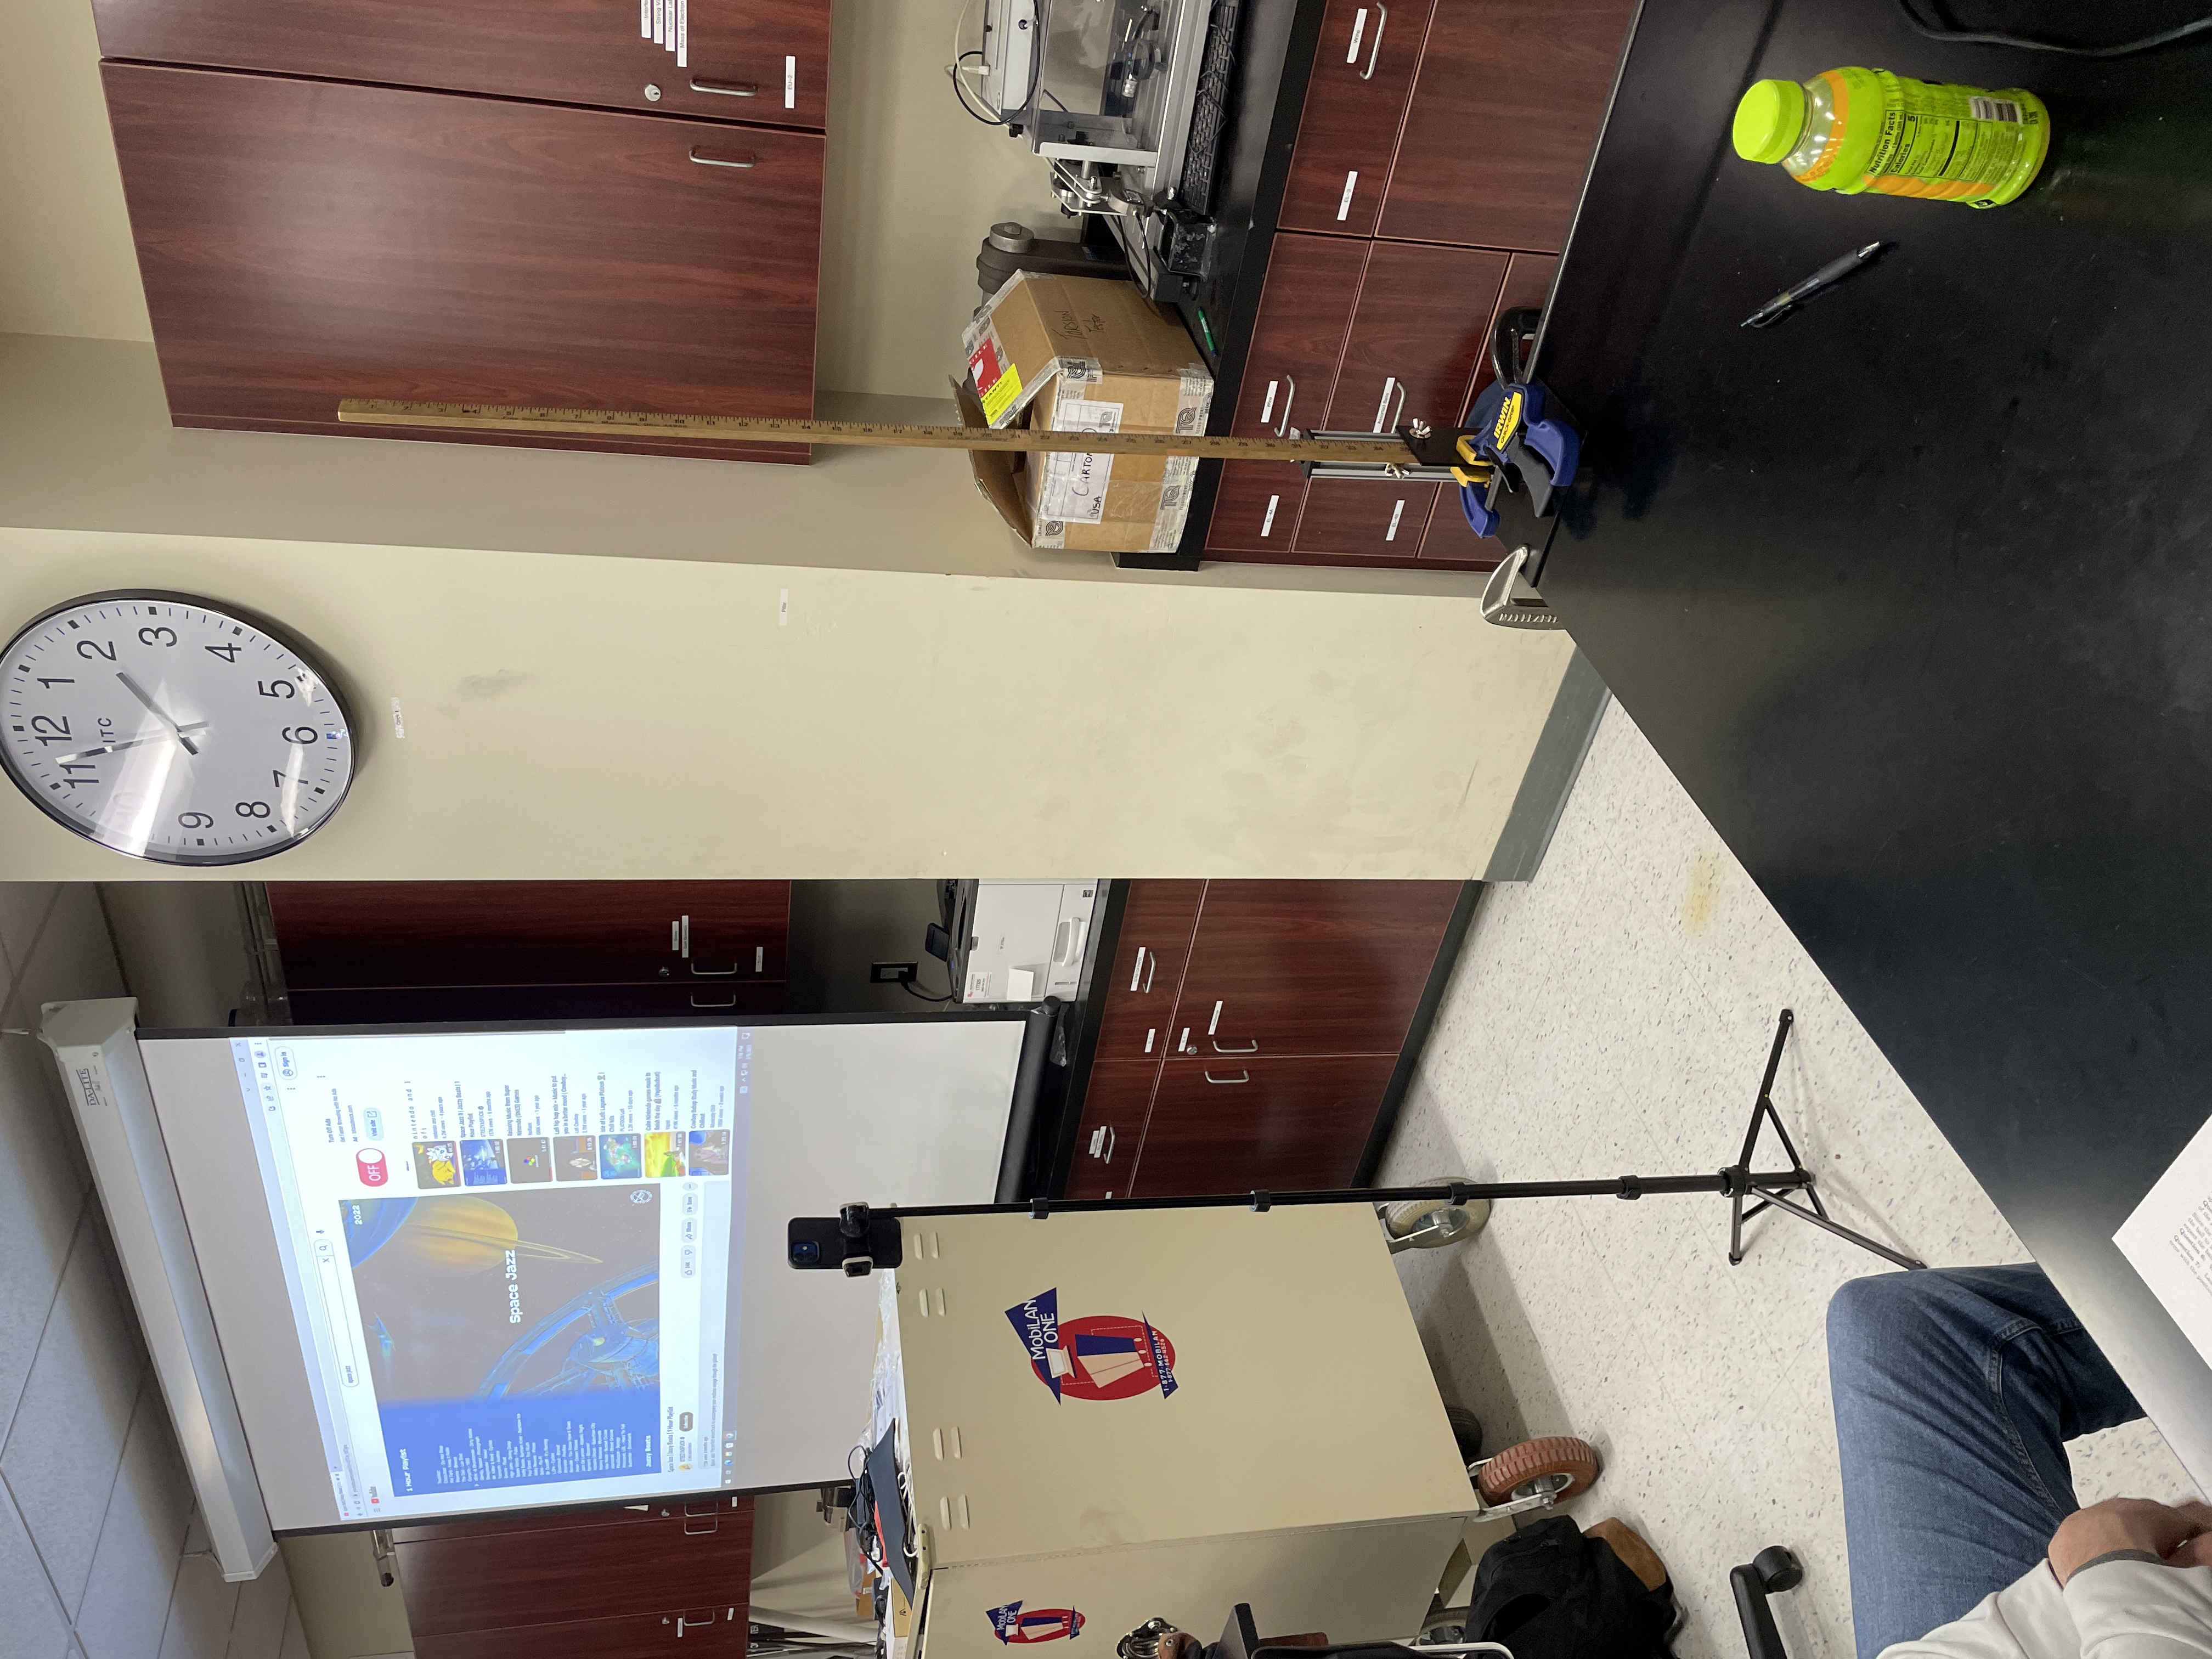
\includegraphics[scale=0.2, angle=-90]{images/IMG_8653.JPG}
    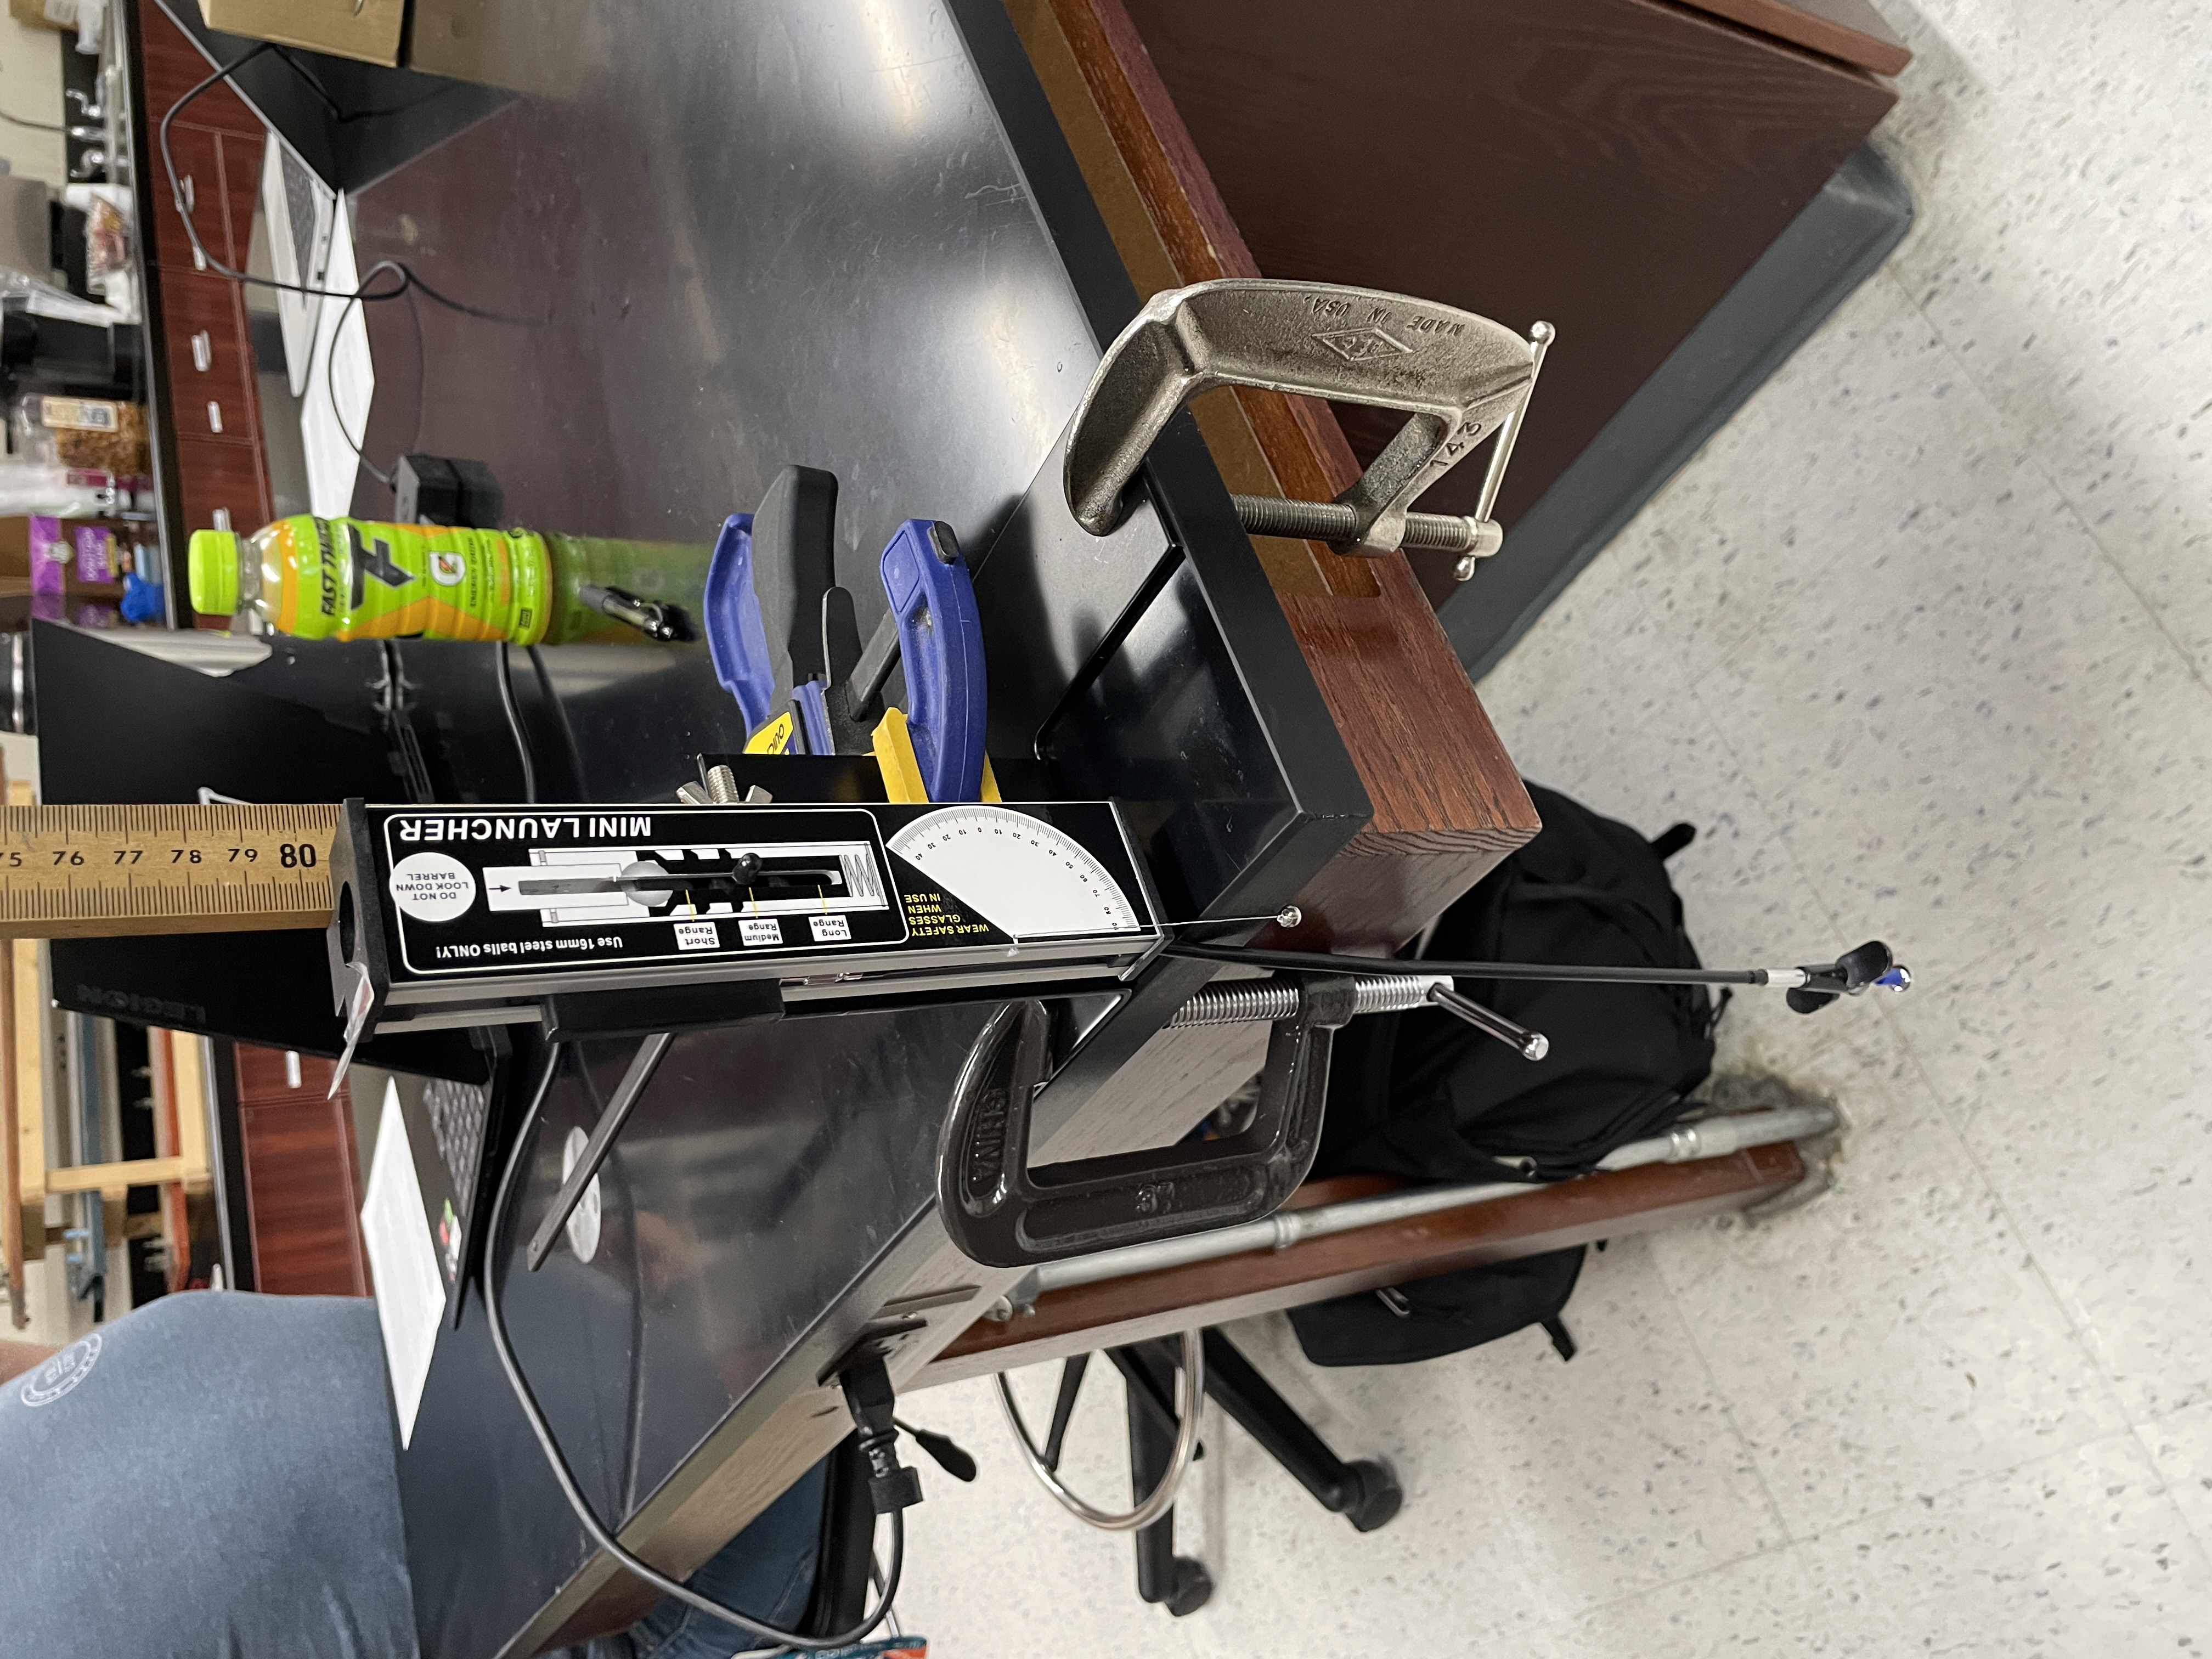
\includegraphics[scale=0.2, angle=-90]{images/IMG_8654.JPG}
    \caption{Images of our setup}
    \label{fig:my_label}
    
\end{figure}

\begin{figure}[H]
    \centering
    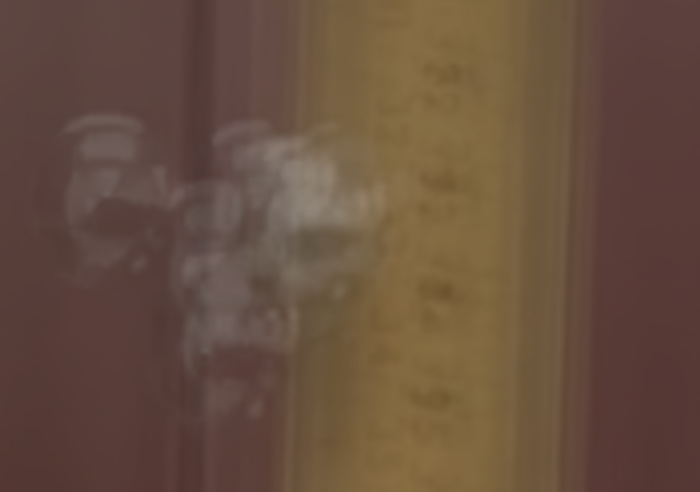
\includegraphics[scale=0.405]{images/10trialsballz.jpg}
    \caption{10 trials stacked on top of each other}
    \label{fig:my_label}
    
\end{figure}

\title{\textbf{\\Height Trials} \textit{(Medium Power)}}

\begin{tabularx}{0.8\textwidth} { 
  | >{$\raggedright\arraybackslash$}X 
  | >{$\centering\arraybackslash$}X 
  | >{$\raggedleft\arraybackslash$}X | }
 \hline
  Trial 1 & 46.0cm \\
 \hline
 Trial 2  & 45.5cm \\
\hline
 Trial 3  & 47.0cm \\
\hline
 Trial 4  & 46.5cm \\
\hline
 Trial 5  & 46.0cm \\
\hline
 Trial 6  & 46.5cm \\
\hline
 Trial 7  & 46.5cm \\
\hline
 Trial 8  & 46.5cm \\
\hline
Trial 9  & 47.0cm \\
\hline
 Trial 10  & 46.0cm \\
\hline
Height_{ave} & 46.35cm \\
\hline
\end{tabularx}

\title{\textbf{\\Height Trials} \textit{(Full Power)}}

\begin{tabularx}{0.8\textwidth} { 
  | >{\raggedright\arraybackslash}X 
  | >{\centering\arraybackslash}X 
  | >{\raggedleft\arraybackslash}X | }
 \hline
 Trial 1 & 84.0 cm \\
 \hline
 Trial 2 & 85.5cm \\
\hline
\end{tabularx}

\title{\textbf{\\Velocity}}

\begin{tabularx}{0.8\textwidth} { 
  | >{\raggedright\arraybackslash}X 
  | >{\centering\arraybackslash}X 
  | >{\raggedleft\arraybackslash}X | }
 \hline
\LARGE \vspace{10pt} V_{ave}  & \begin{equation}
       \sqrt{2(9.8 m/s)(0.475m)}
    \end{equation*} \\
\hline
\LARGE \vspace{10pt} V_{\frac{m}{s}} \vspace{10pt}  & \vspace{10pt} 3.05 m/s \\ 
\hline
\LARGE \vspace{8pt} V_{\frac{mile}{hr}} \vspace{12pt} & \vspace{12pt} 6.82 mi/h \\
\hline
\end{tabularx}
    
\noindent
\title{\textbf{\\Observations}}
\noindent
\begin{list}
    \\ \item - When launching the steel ball vertically, we observed through video and the tracker app that the max height was 83.5cm above the position where the ball was initially launched. This was using the full power of the launcher, and the medium power trials were about half of that.
\end{list}

\newpage

\label{The Experiment Setup}
\subsection*{Range Test}

\noindent
\title{\textbf{Synopsis}}

\begin{list}
 \\ \item - We will find the maximum distance the projectile can travel.
 
 \item - We will set up a launch and landing pad, taking into account our previous measurements, for where we expect the ball to land. 
 
\item - We will record multiple launches and find an average. 
\end{list}

\title{\textbf{\\Range of Projectile}}

\begin{tabularx}{0.8\textwidth} { 
  | >{\raggedright\arraybackslash}X 
  | >{\centering\arraybackslash}X 
  | >{\raggedleft\arraybackslash}X | }
 \hline
 Range & 95cm \\
 \hline
 Jack Height & 100cm \\
 \hline
\end{tabularx}

\title{\textbf{\\Ball Launch Trials \textit{(distance)}}}

\begin{tabularx}{0.8\textwidth} { 
  | >{\raggedright\arraybackslash}X 
  | >{\centering\arraybackslash}X 
  | >{\raggedleft\arraybackslash}X | }
 \hline
 Trial 1 & 97.00cm \\
 \hline
 Trial 2 & 96.70cm \\
 \hline
 Trial 3 & 96.20cm \\
 \hline
 Average & 96.63cm\\
 \hline
 \% Error & \pm 1cm \\
 \hline
\end{tabularx}

\noindent
\title{\textbf{\\Observations}}

\begin{list}
    \\ \item - Through intuition as well as our experiments, we have denounced that we need to launch the ball at 45\textdegree \ in order to get our ball to launch as far as possible in the horizontal direction. 
\end{list}

\newpage

\section*{Soup Can}
\title{\textbf{Objective}}

\begin{list}
\\ \item - Our group will put our skills to the TEST!!! Our objective is to launch the ball and make it land into a soup can on the first try! 

\end{list}

\vspace{5pt}

\noindent
\title{\textbf{Synopsis}}

\begin{list}
\\ \item - We will make calculations and measurements for the height of the launch and the height of the soup can.
 \item - We will find a mathematical expression for the distance the ball travels.
 \item - We will make predictions on where the ball will land based on our calculations and measurements.
 \item - We will now attempt our launch into the soup can, and evaluate what went wrong, if anything.
\end{list}

\title{\textbf{\\Measurements}} 

\vspace{5pt}

\begin{tabularx}{0.8\textwidth} { 
  | >{\raggedright\arraybackslash}X 
  | >{\centering\arraybackslash}X 
  | >{\raggedleft\arraybackslash}X | }
 \hline
 Launch Height & 100cm \\
 \hline
 Can Height & 11.5cm \\
 \hline
 y__{TOT} & 100cm - 11.5cm \\
 \hline
 \vspace{13pt}
 d_{horizontal} & \begin{equation} d = ( 3.05\frac{m}{s} ) \times (\frac{\sqrt{885}}{70}) \end{equation*} \\
 \hline
 First Try? & \checkmark \\
 \hline
\end{tabularx}

\noindent
\title{\textbf{\\Observations}}
\noindent
\begin{list}
    \\ \item - During our first trial, we calculated our trajectory correctly, and we were able to get the steel ball into the soup can from a distance off of a table on our first try. The physics we had calculated held true to what we were learning in class and was very cool to see the equations we had worked so hard for come to fruition in real life.
\end{list}

\newpage
\section*{Target Practice}

\noindent
\title{\textbf{Objective}}

\begin{list}
   \\  \item - Our objective is to utilize what we have learned about the projectile launcher to nail a bullseye on a target with the "long range setting". 
   
\end{list}

\vspace{5pt}
\noindent
\title{\textbf{Synopsis}}

\begin{list}
\\ \item - We will determine the muzzle speed of the "long range" setting.
 \item - We will sketch a drawing of our launch set up.
 \item - We will calculate the necessary angle and distance to hit the      intended target.
 \item - FIRE AWAY! And attempt to hit the mark!
\end{list}

\title{\textbf{\\Measurements}} \vspace{5pt}

\begin{tabularx}{0.8\textwidth} { 
  | >{\raggedright\arraybackslash}X 
  | >{\centering\arraybackslash}X 
  | >{\raggedleft\arraybackslash}X | }
 \hline
 Muzzle Speed & 4.057m/s \\
 \hline
 Distance & 119.11 cm \\
 \hline
 Angle & 30° \\
 \hline
 Result & Failure (embarassing) \\
 \hline
\end{tabularx}

\begin{figure}[H]
    \centering
    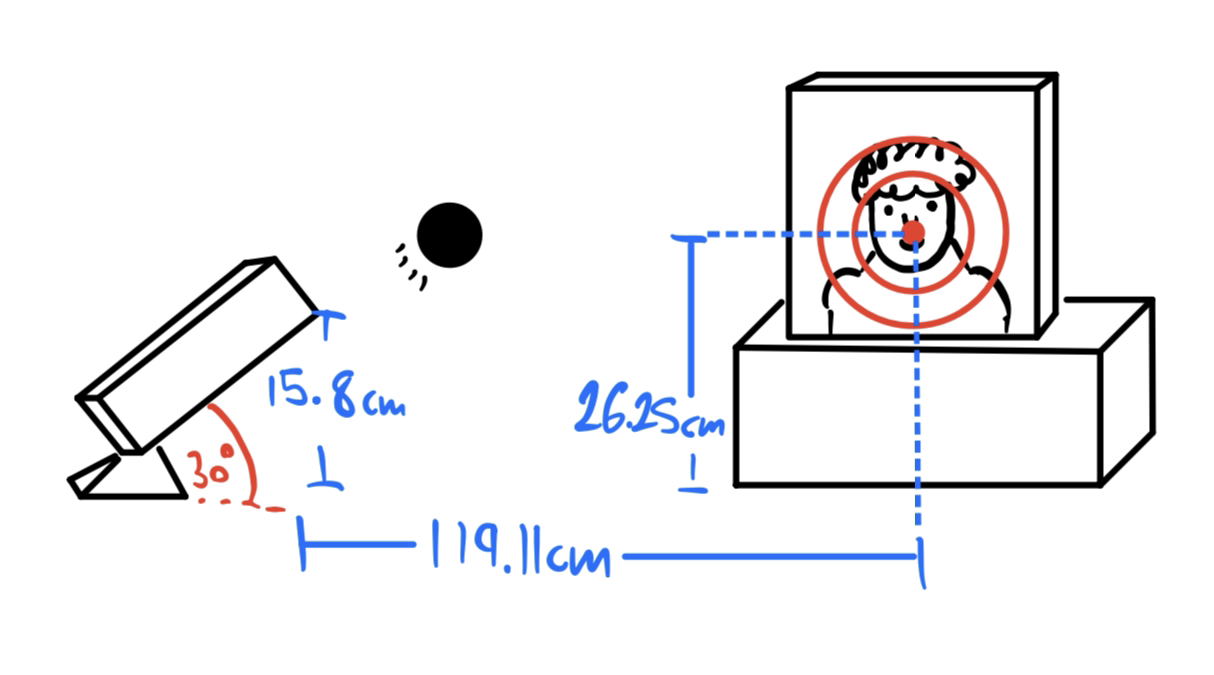
\includegraphics[scale=0.2]{images/ggluis.jpg}
    \caption{Scenario Schematic}
    \label{fig:my_label}
    
\end{figure}



\noindent
\title{\textbf{Observations}}
\begin{list}
    \\ \item - On our first attempt on Luis' face, we completely missed the mark, most likely due to a faulty height calculation. There were also other mechanical errors such as the ball being shot to the right, instead of being shot straight on. 
\end{list}

\section*{Abstract}
\begin{list}
    \\ \item - During our experiments we learned how to link 2D Kinematics to real life. This was achieved by putting our mathmatical skills to the test and then relaying it into the shooting of a metal ball into a soup can on the first try. Next, we attempted to shoot the center of a bullseye from a distance away by only using the kinematics taught in class. 
\end{list}

\end{document}